\documentclass{beamer}
\usepackage{amsmath, amssymb, graphicx}
\usepackage{caption}
\usepackage{tikz}

\usepackage{graphicx}
\usepackage{tabularx}
\usepackage{booktabs}

\title{Differential Privacy : US Broadband Data}
\author{Trishita Patra (MDS202440)}
\institute{Chennai Mathematical Institution}
\date{\today}

\begin{document}
\frame{\titlepage}

% Slide: Background and Motivation
\begin{frame}{ Motivation}
\begin{itemize}
    \item Protecting privacy while performing statistical analysis is quite challenging. 
    \item On one had, the goal of statistics and machine learning is to be as informative as possible. Protecting privacy is the opposite goal.  
    \item Can we protect privacy and still do an informative analysis?
    \item Can you mathematically quantify privacy?
\end{itemize}
\end{frame}


% Slide: Understanding the Eigenimage Representation (1/2)
\begin{frame}{US Internet Usage Data}
\begin{itemize}
    \item This \href{https://archive.ics.uci.edu/dataset/126/internet+usage+data}{\textcolor{blue}{dataset}} contains general demographic information on Internet users in 1997.
    \item 70 variables covering:
    \begin{itemize}
        \item Demographics: Age, Income, Education, Disability
        \item Usage Patterns: Hours online, Activities, Purchase behavior
        \item Attitudes: Censorship opinions
    \end{itemize}
    \item Data files:
    \begin{itemize}
        \item final-general.dat contains demographics of internet usage.
        \item final-general.col contains the variable names for data.
        \item changes contains the conversions from character data to numeric.
    \end{itemize}
    \item Pre-processed numeric encoding (changes file documents categorical→numeric mappings)
\end{itemize}
\end{frame}

\begin{frame}{To Do}
\begin{itemize}
     \item Data Preprocessing 
     \item Identifying PII,QI,Sensitive attributes - Domain Knowledge! 
     \item Developing a suitable Differential Privacy Mechanism.
\end{itemize}
\end{frame}

\begin{frame}{Column Discrepancy}
\begin{itemize}
\item Number of column names: 70
\item Total fields in first row: 72
\end{itemize}
\begin{figure}
    \centering
    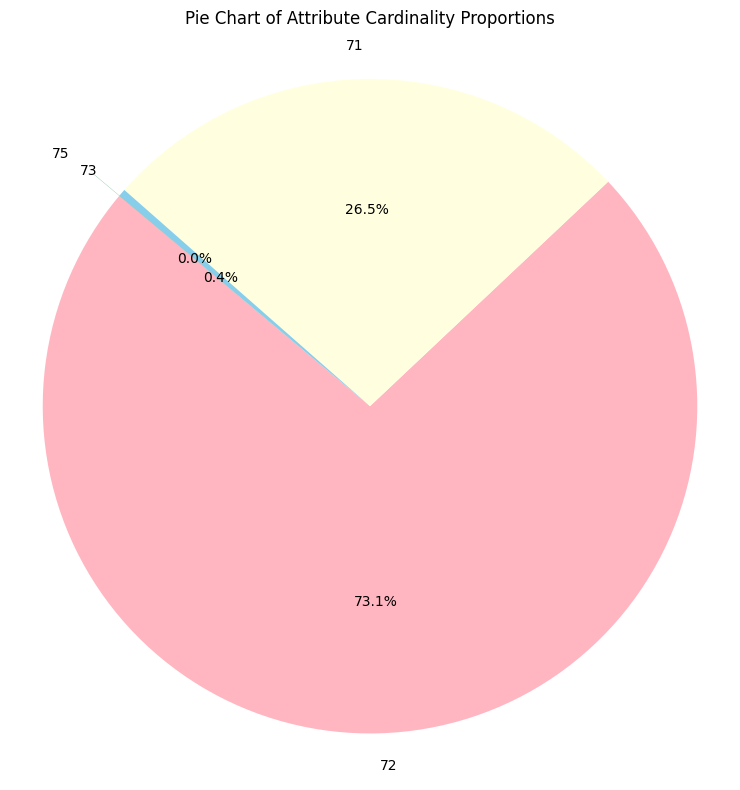
\includegraphics[width=0.6\textwidth]{slide_image/pie.png}
\end{figure}
\end{frame}


% Slide: Updating the Eigenspace
\begin{frame}{Handling Column Discrepancy}
\begin{itemize}
    \item Since percentage of rows with recorded attribute values $>72$ values is very less (~ 0.3761 percent) and less likely to cause substantial loss in understanding the pattern/characteristics of the whole dataset, we eliminate these data points.
    \item Table segregation for analysis:
    \item df1 (71 columns): (2676, 71)
    \item df2 (72 columns): (7390, 72)
\end{itemize}
\end{frame}

\begin{frame}{Handling Column Discrepancy}
\begin{itemize}
    \item Checked for duplicate columns : Absent!
    \item Guesstimating missing attribute names!
\end{itemize}
\end{frame}

\begin{frame}{Guesstimate!}
\begin{itemize}
    \item Looked at Column cardinality.
    \item In both datasets, max column cardinality = no. of datapoints $>$
    \item Unique ID identified! 
    \item Column indices found. 71 attributes!
\end{itemize}
\end{frame}
\begin{frame}{Guesstimate : The Big Assumptions}
\begin{itemize}
    \item  With respect to df2, df1 has missing values from a single column only.
    \item The underlying cause of the missing values do not affect other attributes. i.e. if Column A is taking n many values in df1, it is taking ~n (almost n many) values in df2 as well.
\end{itemize}
\end{frame}

\begin{frame}{Guesstimating the unknown column of df2}
\begin{figure}
    \centering
    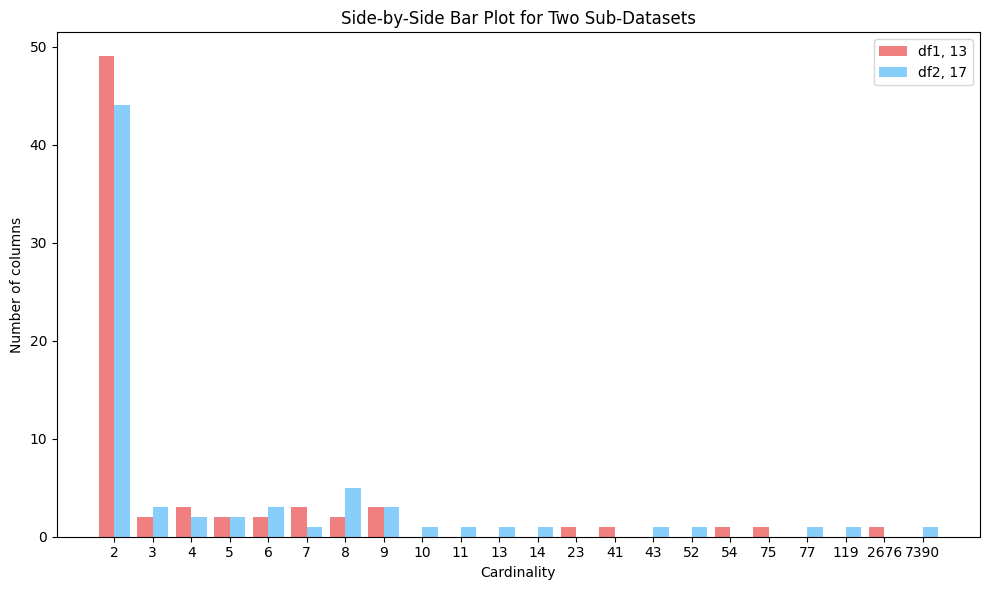
\includegraphics[width=1.0\textwidth]{slide_image/bar_col.png}
\end{figure}
\end{frame}

\begin{frame}{Guesstimating the unknown column of df2}
\begin{figure}
    \centering
    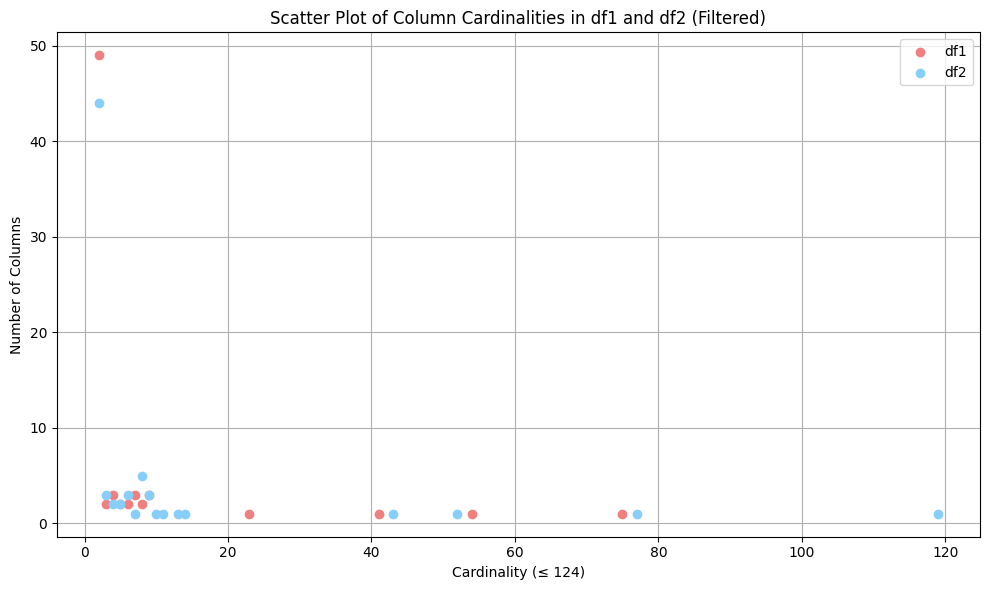
\includegraphics[width=1.0\textwidth]{slide_image/scat_col.png}
\end{figure}
\end{frame}

\begin{frame}{Guesstimate}
\begin{itemize}
    \item Now see that there are total five column cardinality $> 45$, but $< 124$. With our assumption, it is reasonable that following two column cardinality pairs in (df1,df2) correspond to same recorded attribute : (54,52) and (75,77)
    \item column cardinality 119 (which has to be states) in df2 is the unknown one!
    \item column dropped from df2.
    \item dimensionality matched ! (10066, 71)
\end{itemize}
\end{frame}

\begin{frame}{Differential Privacy}
\begin{itemize}
    \item Differential privacy mathematically guarantees that anyone seeing theresult of a differentially private analysis will essentially make the same
inference about any individual’s private information, whether or not that
individual’s private information is included in the input to the analysis.
    \item It works by adding noise to/randomizing the sensitive
values to protect privacy, while maximizing the accuracy
of queries.
\item Domain knowledge helps us to predict which queries might be executed on the dataset.
\end{itemize}
\end{frame}

\begin{frame}{Identifying Column Types}
 Based on domain Knowledge and column cardinality, we determine
\begin{itemize}
    \item PII (Personally Identifiable Information) : Attributes that can uniquely or directly identify an individual.
\item Quasi-Identifiers (QI) : Attributes that don’t identify directly but can be combined to do so.
\item Sensitive Attributes : Attributes a user would consider private or are policy-sensitive.
\item Non-sensitive : None of the above.
\end{itemize}
\end{frame}

\begin{frame}{Attribute Distribution}
\begin{figure}
    \centering
    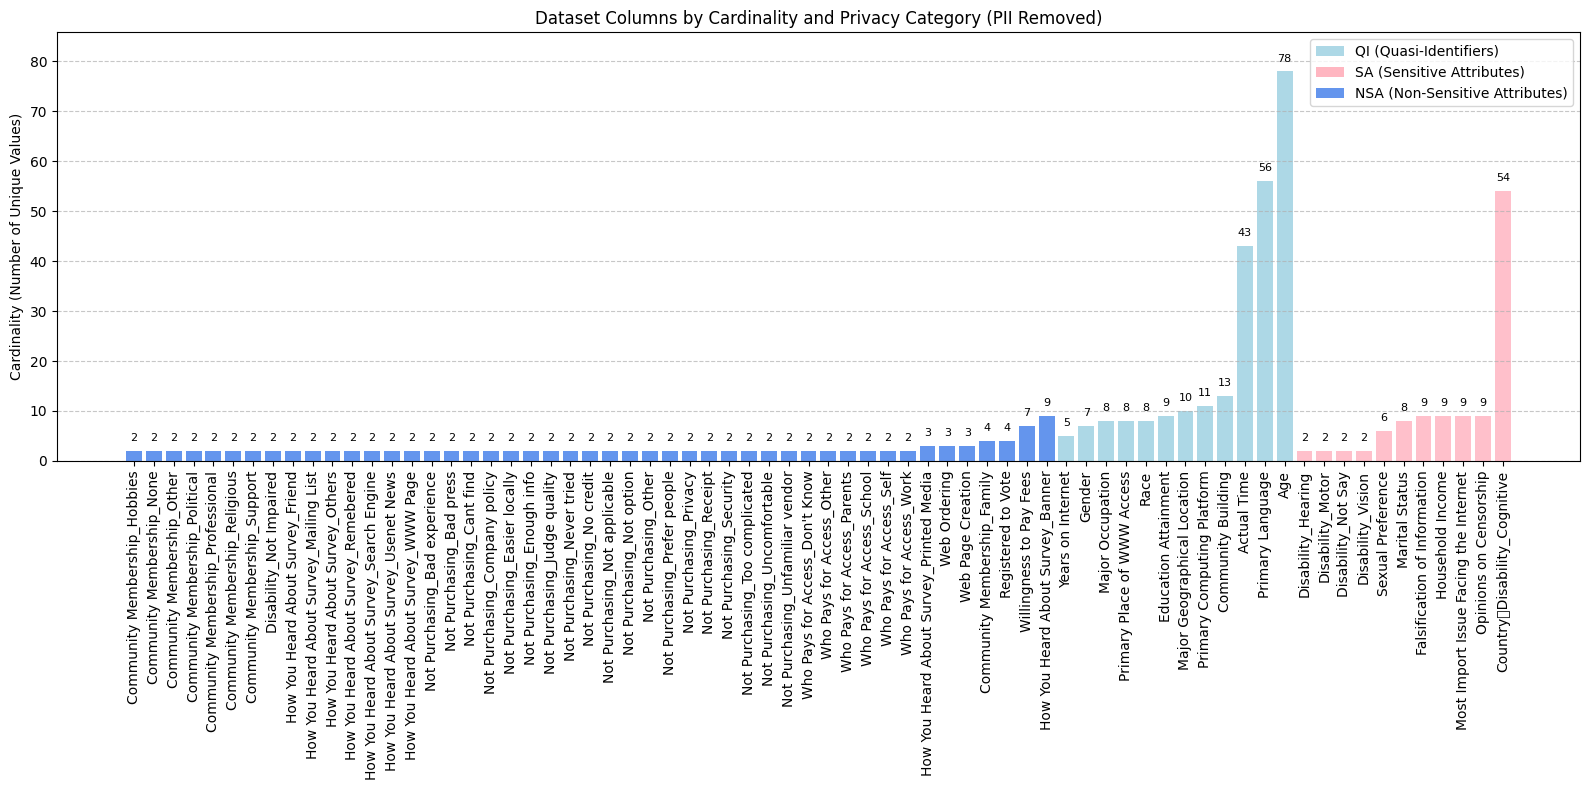
\includegraphics[width=1.06\textwidth]{slide_image/col_type.png}
\end{figure}
\end{frame}

\begin{frame}{Attribute Distribution (n=71)}
\begin{table}[h]
\centering
\small % Reduce font size
\begin{tabular}{|l|c|}
\hline
\textbf{Category} & \textbf{Count (\%)} \\ \hline
PII & 1 (1.4\%) \\ \hline
Quasi-Identifiers (QI) & 12 (16.9\%) \\ \hline
Sensitive Attributes (SA) & 11 (15.5\%) \\ \hline
Non-Sensitive (NSA) & 47 (66.2\%) \\ \hline
\end{tabular}
\end{table}

\vspace{0.5em}
\begin{itemize}
\item \textbf{PII}: Removed entirely
\item \textbf{QI}: Generalization/bucketing applied
\item \textbf{SA}: Differential privacy mechanisms
\item \textbf{NSA}: Preserved as-is
\end{itemize}
\end{frame}

\begin{frame}{Attribute Distribution : Ratio}
\begin{figure}
    \centering
    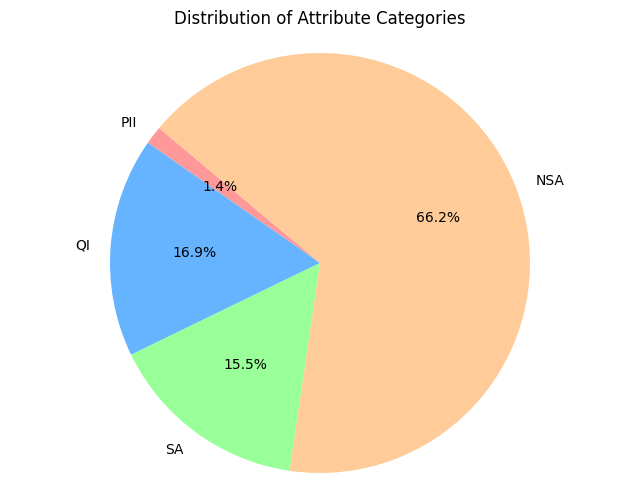
\includegraphics[width=1\textwidth]{slide_image/cat_dist.png}
\end{figure}
\end{frame}

\begin{frame}{Randomized Response Implementation}
\footnotesize

\begin{block}{Core Mechanism}
\begin{enumerate}
\item For each sensitive column:
\begin{itemize}
\item Calculate truth probability: 
\vspace{-0.5em}
\[ p = \frac{e^\epsilon}{e^\epsilon + k - 1} \quad (k=\text{\# categories}) \]
\end{itemize}

\item Generate perturbation mask:
\begin{lstlisting}[language=Python]
mask = np.random.random(len(df)) < p  # True=keep, False=perturb
\end{lstlisting}

\item Apply randomization: Among lies
\end{enumerate}
\end{block}

\begin{exampleblock}{Key Properties}
\begin{itemize}
\item Satisfies $\epsilon$-DP: $\frac{p}{q} = e^\epsilon$ where $q=\frac{1-p}{k-1}$
\item Runtime: $\mathcal{O}(n)$ per column
\item Space: $\mathcal{O}(1)$ beyond original data
\end{itemize}
\end{exampleblock}
\end{frame}

\begin{frame}{Randomized Response Privacy Guarantees}
\footnotesize

\textbf{DP Proof}:
For any $x,y \in$ domain:
\[
\frac{\Pr[\text{Output}=x|\text{True}=x]}{\Pr[\text{Output}=x|\text{True}=y]} = \frac{p}{q} = e^\epsilon
\]
where:
\begin{itemize}
\item $p = \frac{e^\epsilon}{e^\epsilon + k - 1}$ (truth probability)
\item 1-p is total lie probability
\item $q = \frac{1}{e^\epsilon + k - 1}$ (per-lie probability)
\end{itemize}

\vspace{0.5em}
\textbf{Intuition}:
\begin{itemize}
\item $\epsilon \to 0$: $p\to\frac{1}{k}$ (max privacy)
\item $\epsilon \to \infty$: $p\to1$ (no privacy)
\end{itemize}
\end{frame}


\begin{frame}{Accuracy vs. Privacy}
\begin{figure}
    \centering
    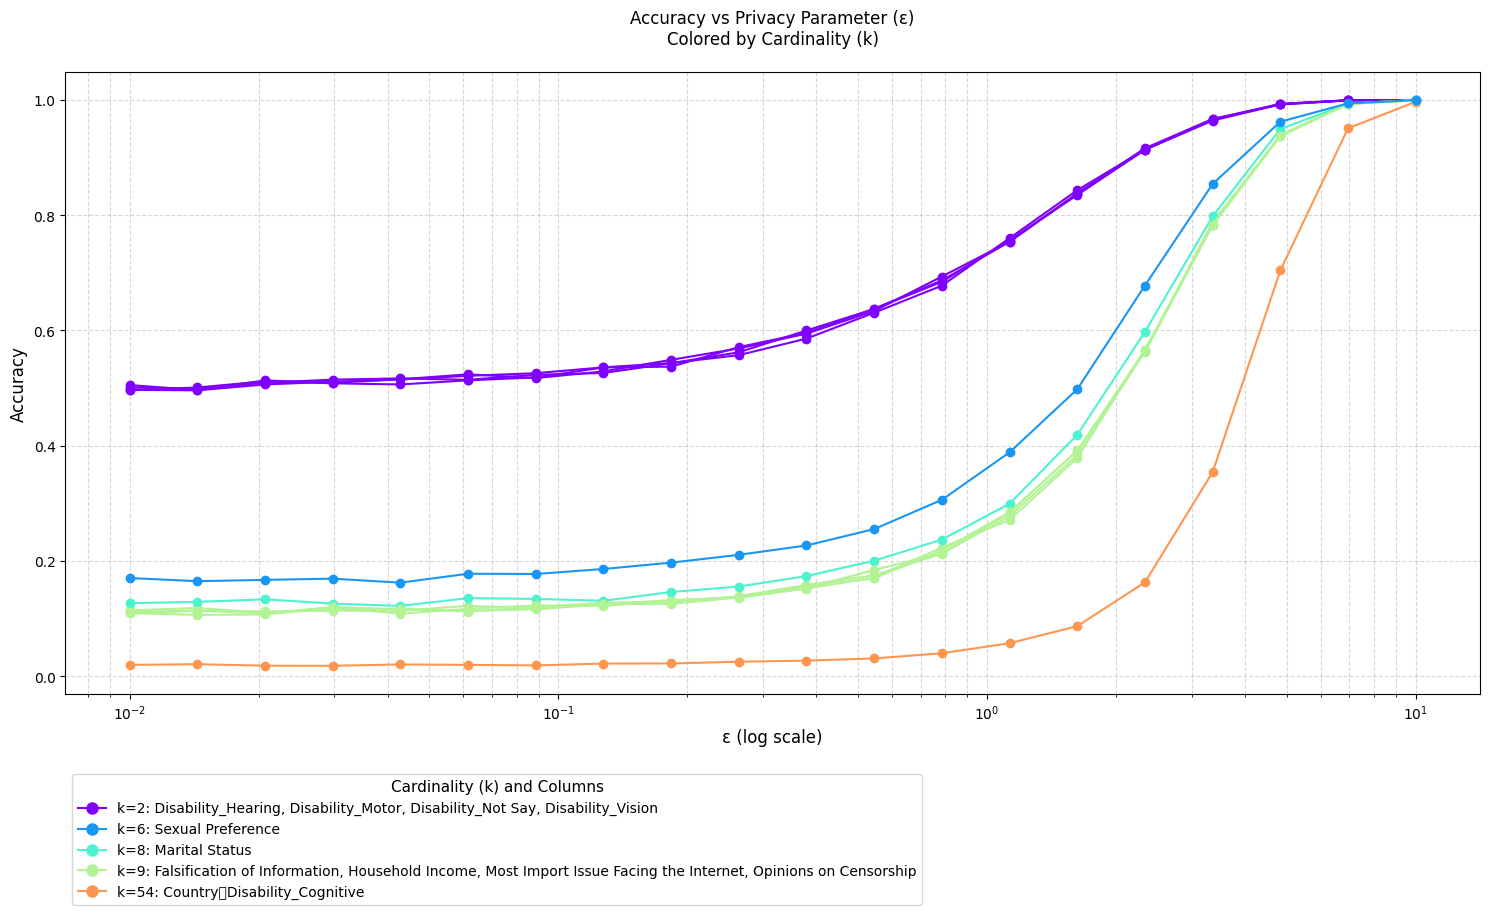
\includegraphics[width=1.06\textwidth]{slide_image/final.png}
\end{figure}
\end{frame}

\begin{frame}{Key Observations}
\footnotesize

\begin{block}{Privacy vs. Accuracy Tradeoff}
\begin{itemize}
\item Higher values of $\epsilon$ (less privacy) lead to higher truth probability $p$, resulting in higher accuracy
\item Lower values of $\epsilon$ (stronger privacy) increase randomization, leading to lower accuracy
\end{itemize}
\end{block}

\begin{block}{Impact of Cardinality ($k$)}
\begin{itemize}
\item Fewer categories (lower $k$) yield higher $p$ for the same $\epsilon$, producing higher accuracy
\begin{itemize}
\item Example: Binary data ($k=2$) is easier to protect than 10-category data
\end{itemize}
\item More categories (higher $k$) require larger $\epsilon$ values to maintain usable accuracy
\end{itemize}
\end{block}
\end{frame}

\begin{frame}{Comparison of Distribution of Sensitive Attributes }
\begin{figure}
    \centering
    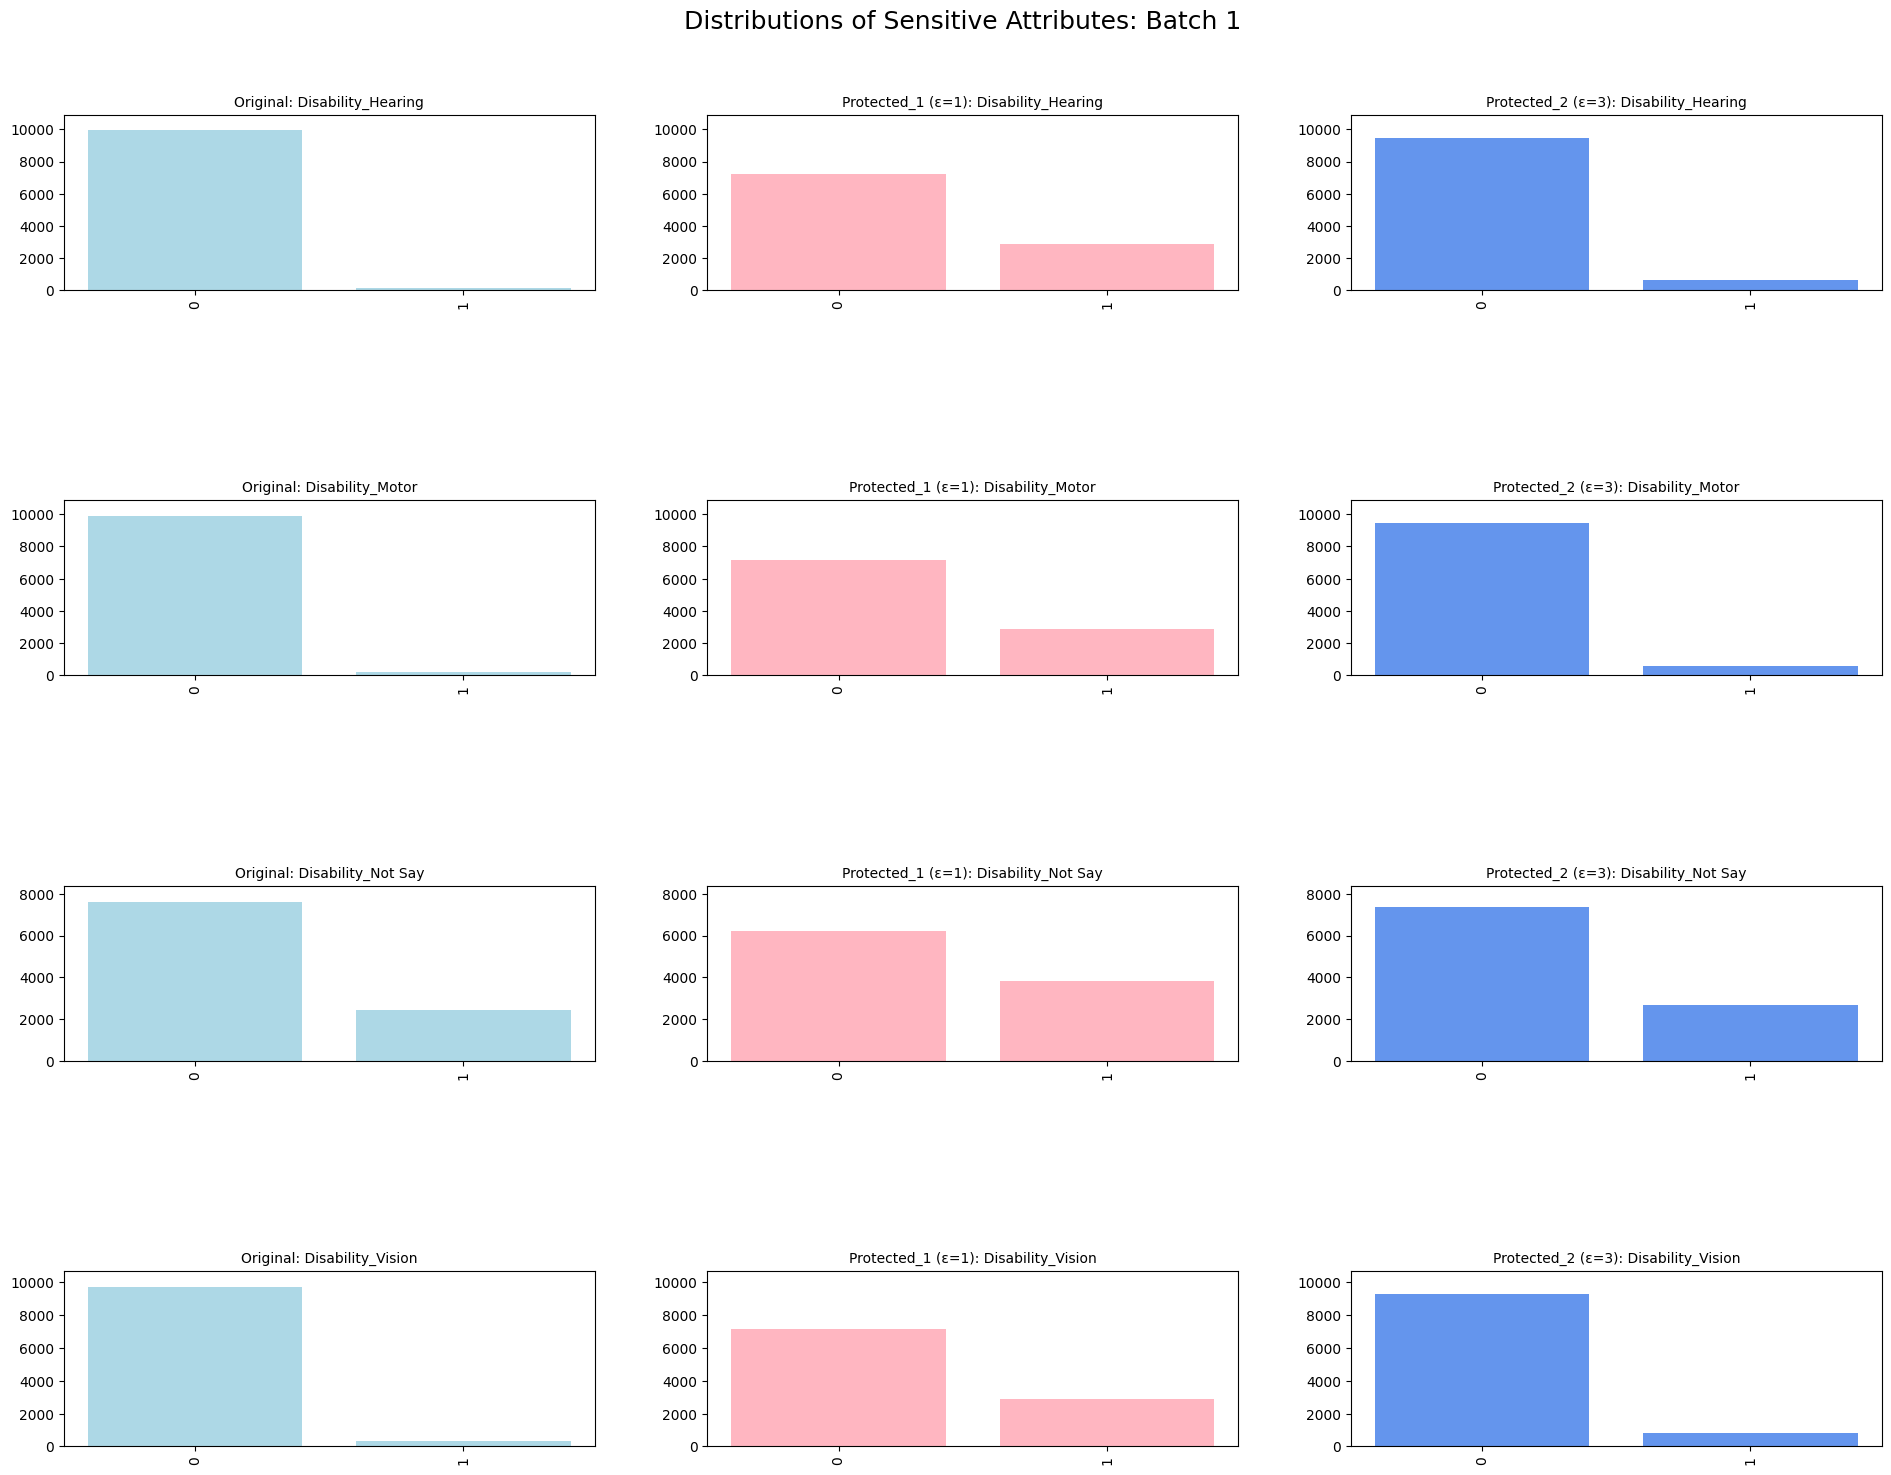
\includegraphics[width=1\textwidth]{final_2_1.png}
\end{figure}
\end{frame}


\begin{frame}{Comparison of Distribution of Sensitive Attributes }
\begin{figure}
    \centering
    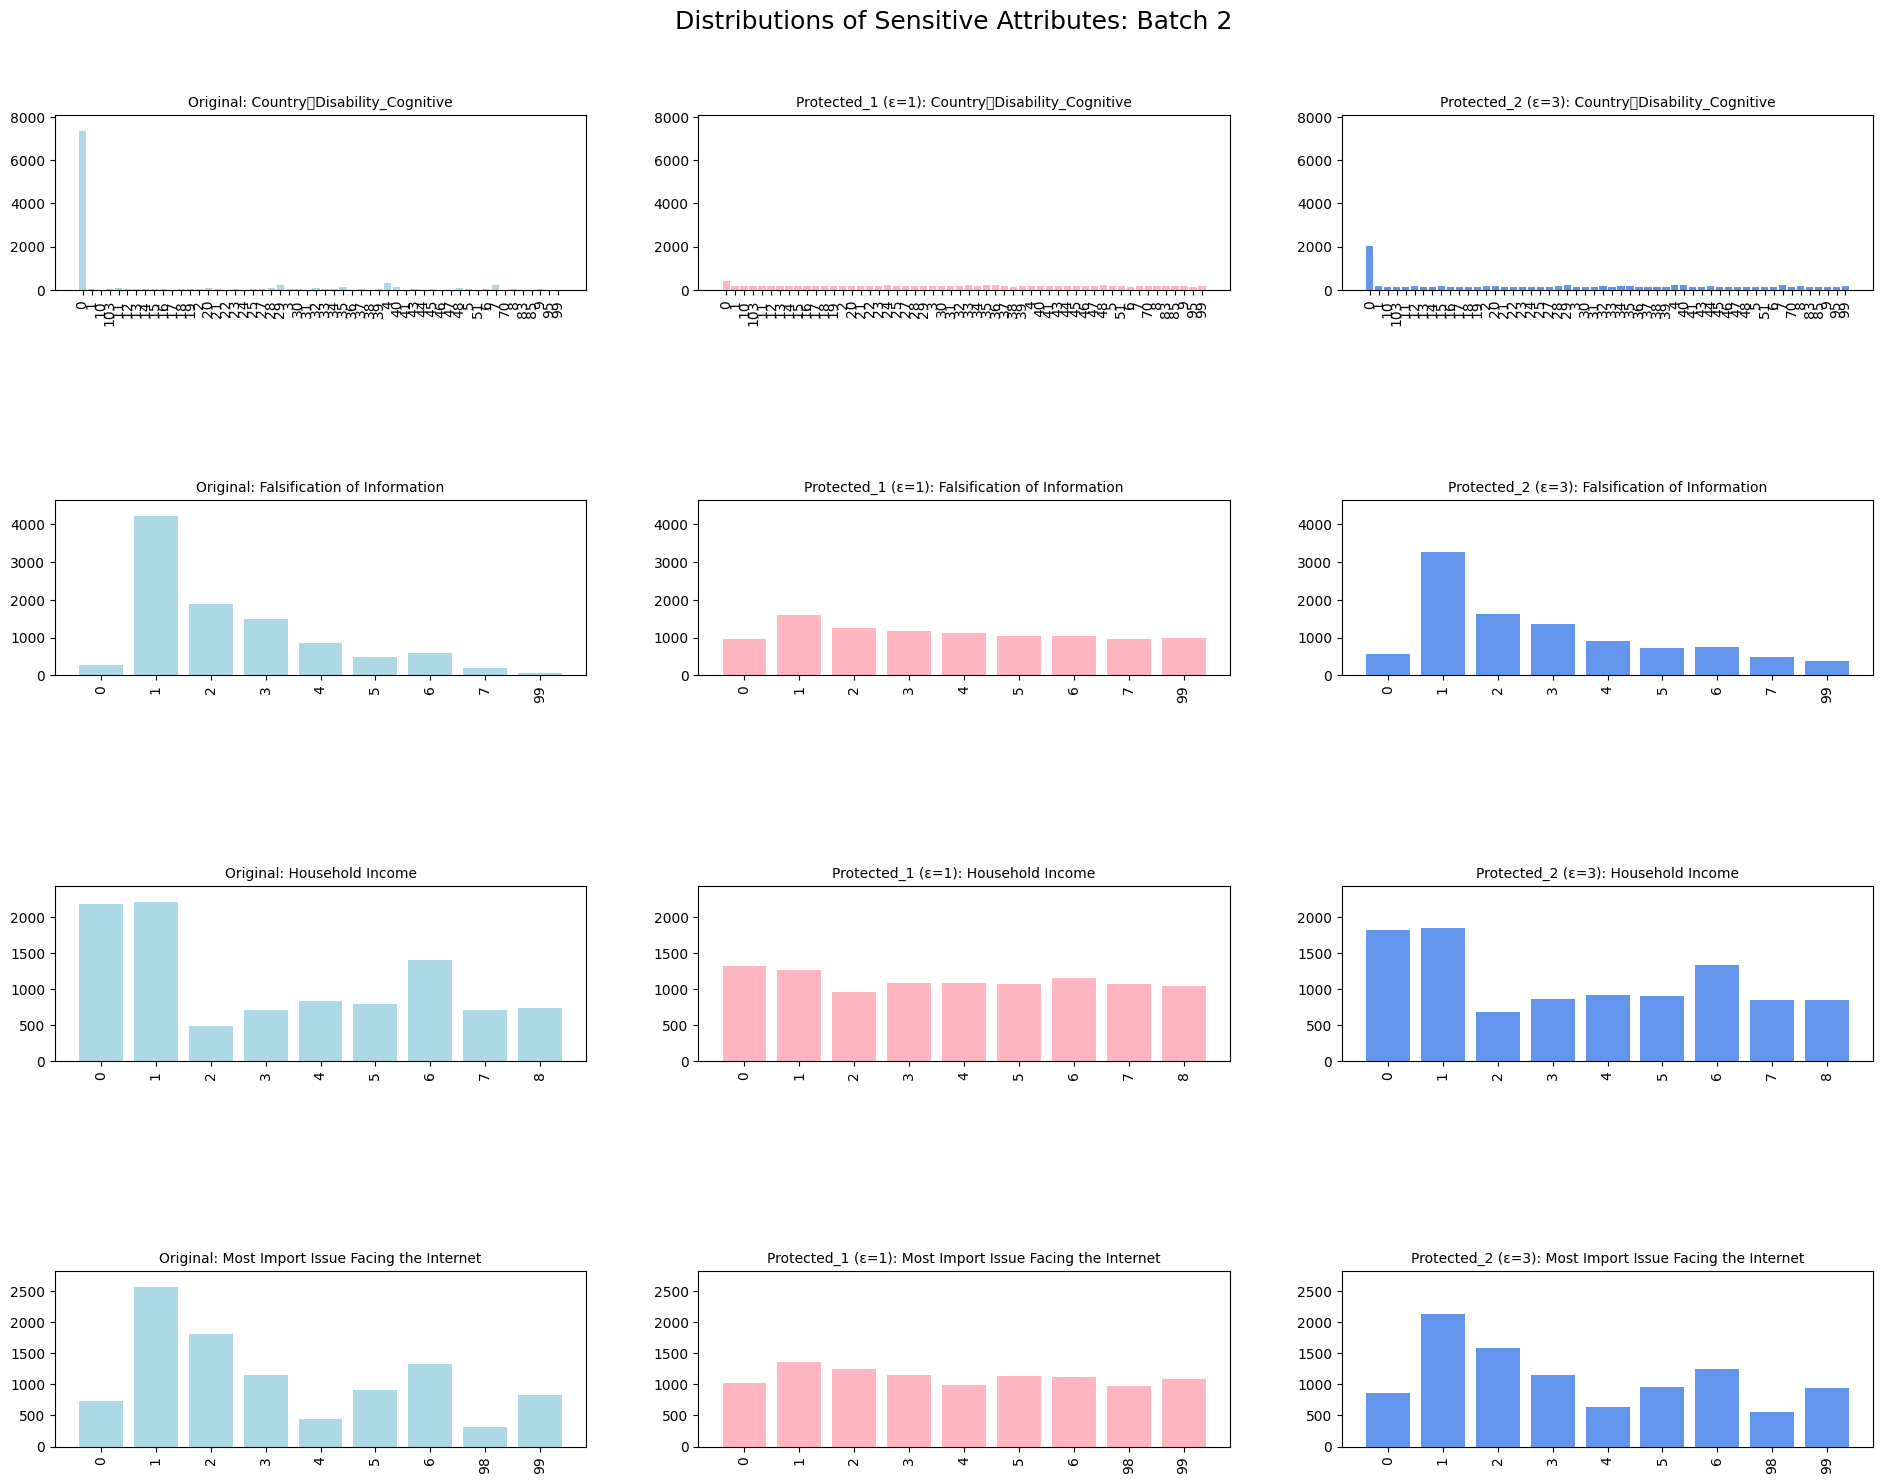
\includegraphics[width=1\textwidth]{final_2_2.png}
\end{figure}
\end{frame}

\begin{frame}{Comparison of Distribution of Sensitive Attributes }
\begin{figure}
    \centering
    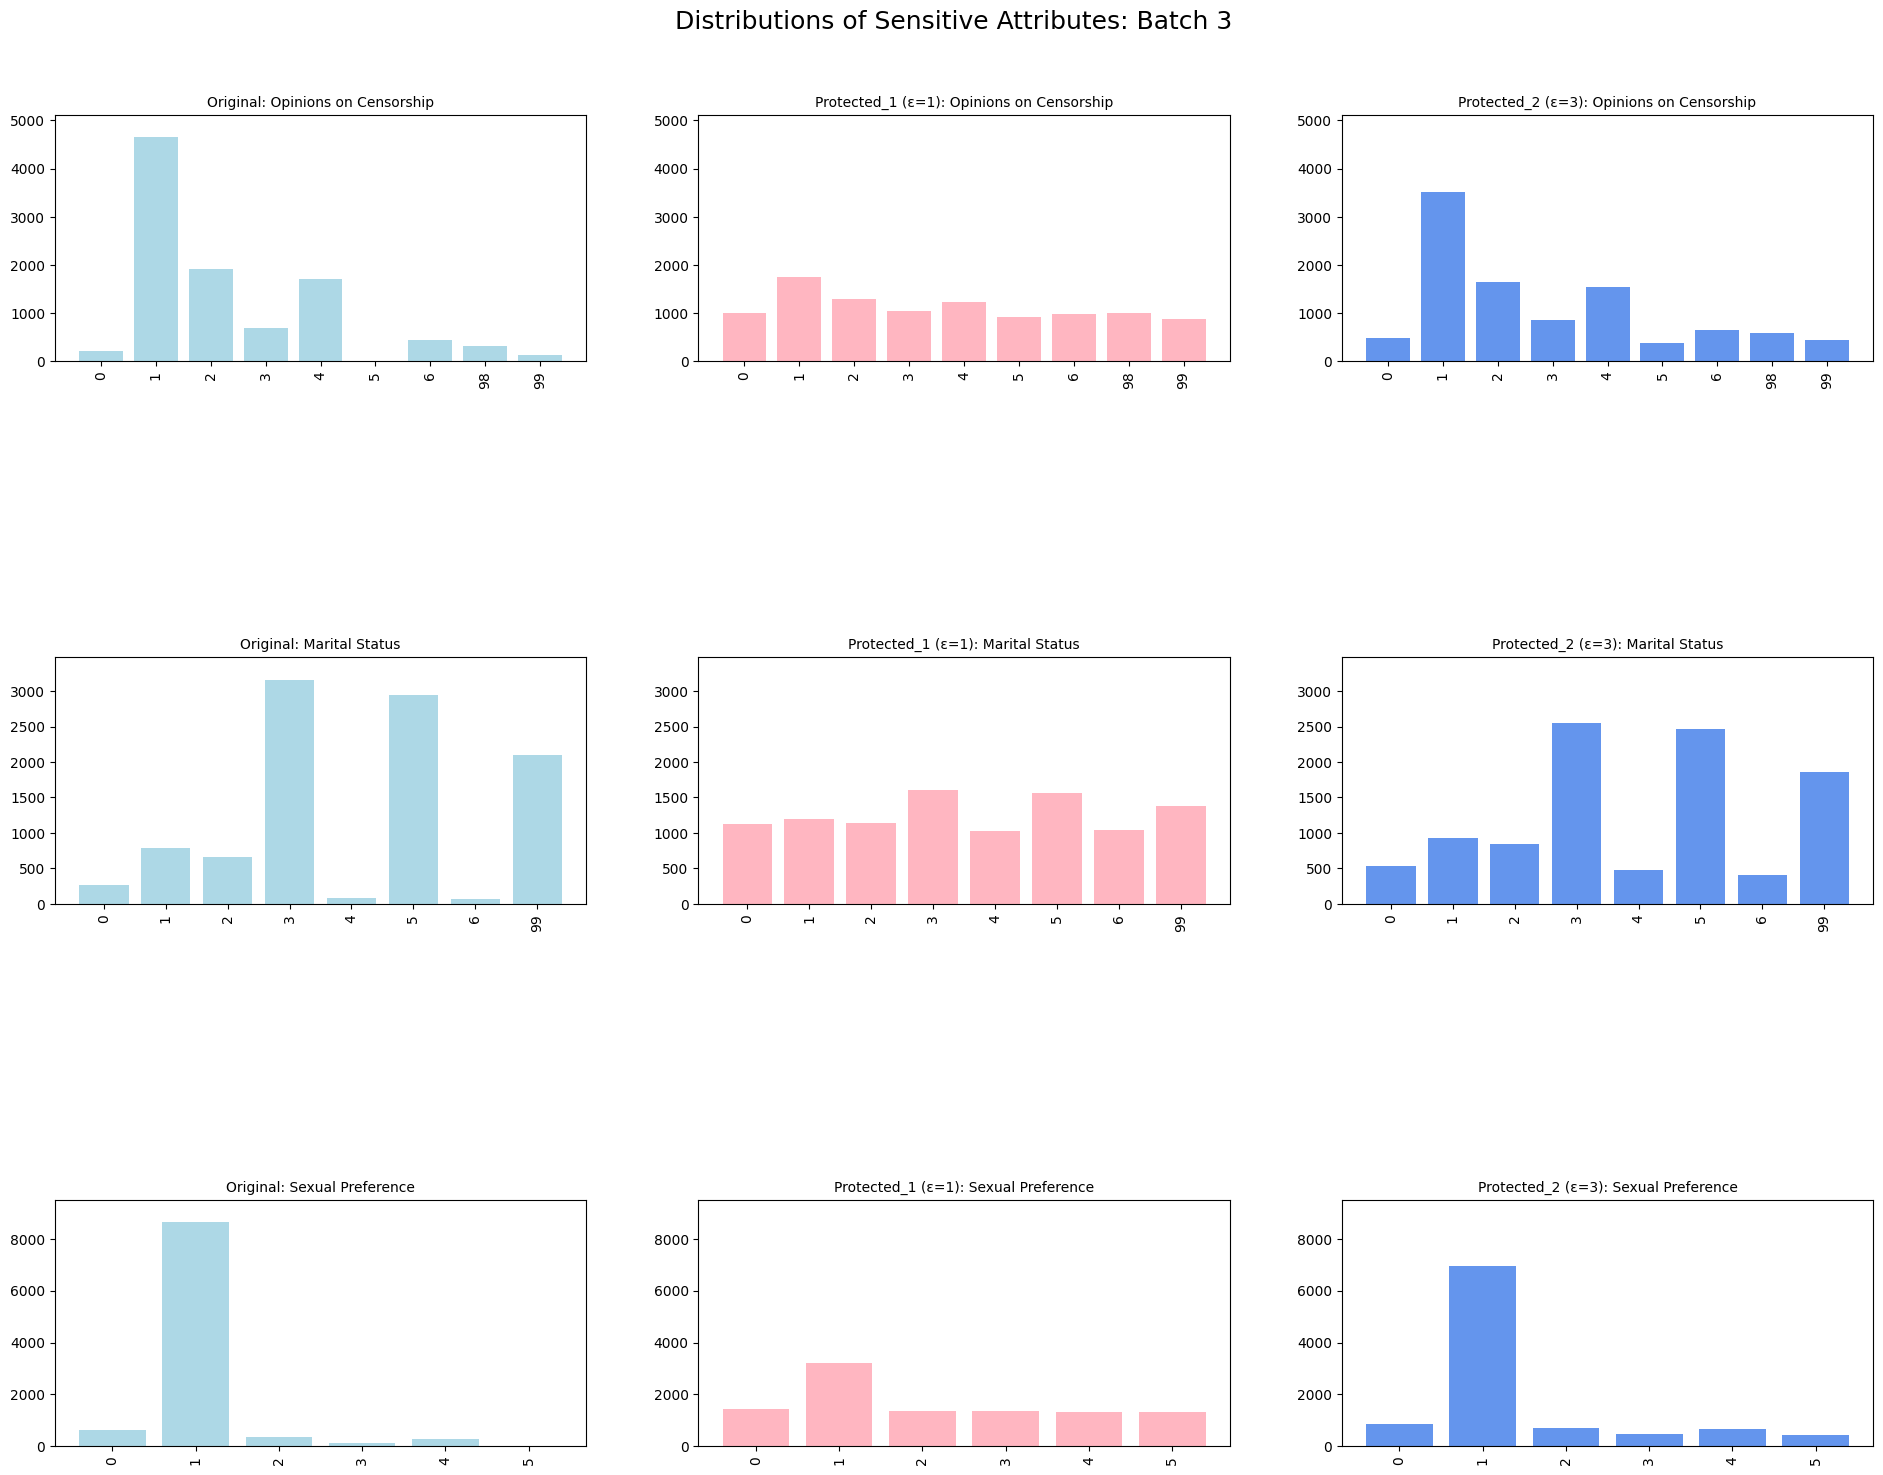
\includegraphics[width=1\textwidth]{final_2_3.png}
\end{figure}
\end{frame}

\begin{frame}{Conclusion}

Differential privacy via randomized response provides a mathematically rigorous way to trade accuracy for privacy in categorical data. The key parameters are:
\begin{itemize}
\item Privacy parameter ($\epsilon$): Controls the noise-accuracy balance.
\item Cardinality (k): Determines how much noise is needed.
\end{itemize}

\begin{alertblock}{Sensitive Attribute Distribution}
\begin{itemize}
\item With increasing $\epsilon$, the protected data distribution converges to the original distribution
\item This convergence occurs regardless of attribute cardinality
\end{itemize}
\end{alertblock}

\begin{alertblock}{Implementation Guidance}
\begin{itemize}
\item Preprocess high-$k$ features (bucket/group)
\item Choose $\epsilon$ based on data sensitivity
\end{itemize}
\end{alertblock}

By carefully selecting $\epsilon$ and preprocessing high-cardinality features, practitioners can achieve meaningful privacy guarantees while preserving data utility.

\end{frame}

\begin{frame}
\centering{\LARGE{Thank You!}}

\end{frame}

\end{document}
